\documentclass{bjt}
% more options
% \documentclass[12pt]{bjt}
% by default 10pt, 16:9 aspect ratio

\usepackage{listings}
\definecolor{codegreen}{rgb}{0,0.6,0}
\definecolor{codegray}{rgb}{0.5,0.5,0.5}
\definecolor{codepurple}{rgb}{0.58,0,0.82}
\definecolor{backcolour}{rgb}{0.95,0.95,0.92}

\lstdefinestyle{bjt}{
    language=Python,
    backgroundcolor=\color{backcolour},
    commentstyle=\color{codegreen},
    keywordstyle=\color{magenta},
    numberstyle=\tiny\color{codegray},
    stringstyle=\color{codepurple},
    basicstyle=\rmfamily\footnotesize\slshape,
    breakatwhitespace=false,
    breaklines=true,
    captionpos=b,
    keepspaces=true,
    numbers=left,
    numbersep=5pt,
    showspaces=false,
    showstringspaces=false,
    showtabs=false,
    tabsize=2,
    frame=single,
    framesep=2pt,
    framerule=0.2pt,
    rulecolor=\color{black},
}

\lstset{style=bjt}


% Presentation information
\newcommand{\Title}{ORM Methods}                                          % (EDIT HERE)
\newcommand{\ShortTitle}{ORM Methods}                                     % (EDIT HERE) short form for footer
\newcommand{\Subtitle}{Odoo 17 Development Tutorials}                     % (EDIT HERE)
\newcommand{\AuthorName}{Ahmed Muhumed}                                   % (EDIT HERE)
\newcommand{\ShortAuthor}{Ahmed M.}                                       % (EDIT HERE) short form for footer
\newcommand{\PresentationDate}{\today}                                    % (EDIT HERE)
\serieslabel{Odoo Developer Program}                                      % (EDIT HERE) small label above title; leave empty to hide


% Beamer metadata
\title[\ShortTitle]{\Title}               % (DO NOT EDIT HERE)
\subtitle{\Subtitle}                      % (DO NOT EDIT HERE)
\author[\ShortAuthor]{\AuthorName}         % (DO NOT EDIT HERE)
\date{\PresentationDate}                  % (DO NOT EDIT HERE)

% for directory structure making
\usepackage[edges]{forest}

\begin{document}

% make title frame
\maketitleframe

% make table of contents frame
\begin{frame}{Outline}
\begin{columns}[T]
\begin{column}{0.48\textwidth}
\tableofcontents[sections={1-11}]
\end{column}
\begin{column}{0.48\textwidth}
\tableofcontents[sections={12-21}]
\end{column}
\end{columns}
\end{frame}

% content start
% =========================================================
% 1. Introduction to ORM Methods
% =========================================================
\section{Introduction to ORM Methods}

\begin{frame}[standout]
  Introduction to ORM\\Methods
\end{frame}

\begin{frame}[fragile]{WHAT IS ORM?}
  \begin{itemize}
    \item The ORM stands for \textbf{Object Relational Mapping}.
    \item It is a programming technique that allows developers to interact with a
          database using Python objects and methods instead of writing SQL queries
          \textbf{directly}.
    \item In Odoo, the ORM acts as a bridge between the Python application and the
          PostgreSQL database.
    \item Instead of writing:
  \end{itemize}
\begin{lstlisting}[language=SQL]
INSERT INTO student_student (name, age) VALUES ('Ahmed', 22);
\end{lstlisting}
  \begin{itemize}
    \item we simply write:
  \end{itemize}
\begin{lstlisting}
self.env['student.student'].create({
    'name': 'Ahmed',
    'age': 22,
})
\end{lstlisting}
\end{frame}

\begin{frame}[fragile]{WHAT DOES ``OBJECT RELATIONAL MAPPING'' MEAN?}
  \begin{itemize}
    \item The term consists of three parts.
  \end{itemize}
  \begin{enumerate}
    \item \textbf{Object} -- an object is an instance of a Python class.
\begin{lstlisting}
student = self.env['student.student'].browse(1)
\end{lstlisting}
          Here, \texttt{student} is a Python object representing a student.
    \item \textbf{Relational} -- a relational database stores data in tables that are
          connected using relationships.\\[0.2em]
          Students $\leftrightarrow$ Classes \quad (e.g.\ Mohamed $\leftrightarrow$ Grade 12)
    \item \textbf{Mapping} -- mapping means connecting two different worlds.\\[0.2em]
          Python Object $\Rightarrow$ Odoo ORM $\Rightarrow$ PostgreSQL Table
  \end{enumerate}
\end{frame}

\begin{frame}{ORM ARCHITECTURE}
  \begin{center}
    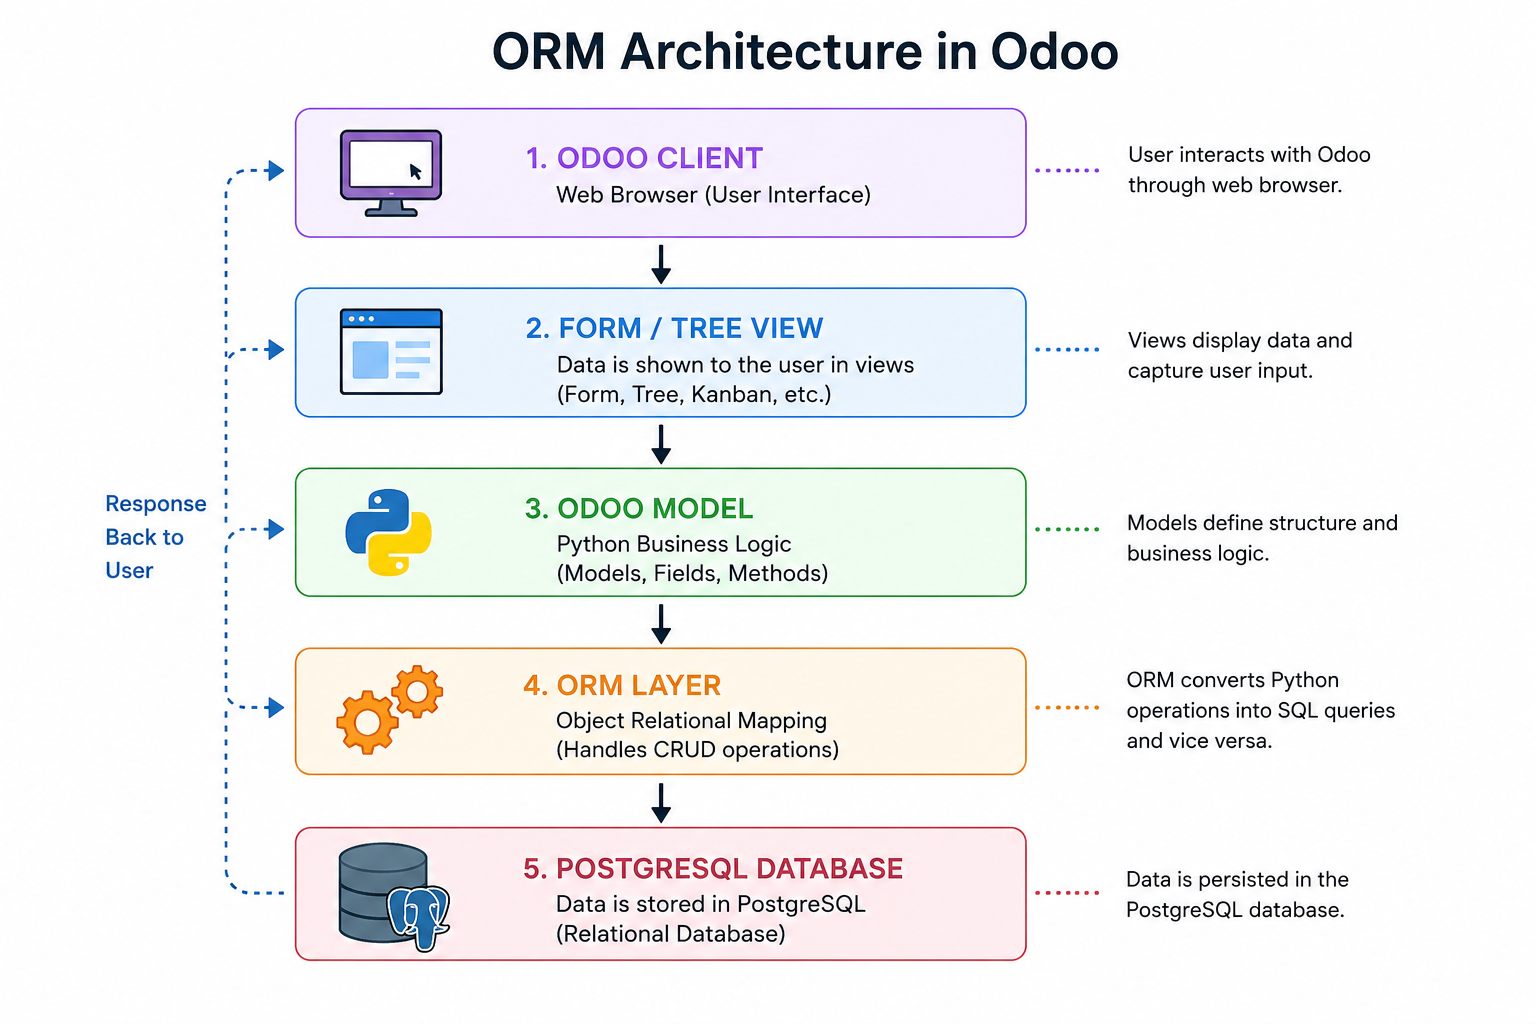
\includegraphics[width=0.92\textwidth,height=0.78\textheight,keepaspectratio]{assets/orm_architecture.png}
  \end{center}
\end{frame}

\begin{frame}{WHY IS ORM IMPORTANT?}
  \begin{itemize}
    \item Without an ORM, developers would need to:
      \begin{itemize}
        \item Write SQL for every operation.
        \item Manage database connections manually.
        \item Convert database rows into Python objects.
        \item Prevent SQL injection.
      \end{itemize}
    \item Although powerful, the ORM has limitations.
      \begin{itemize}
        \item Less control over complex SQL queries.
        \item Very large reports may require raw SQL.
        \item Advanced database tuning sometimes needs direct SQL.
      \end{itemize}
  \end{itemize}
\end{frame}

\begin{frame}{COMMON ORM METHODS}
  \begin{columns}[T]
    \begin{column}{0.48\textwidth}
      \begin{itemize}
        \item \texttt{create}
        \item \texttt{write}
        \item \texttt{unlink}
        \item \texttt{copy}
        \item \texttt{exists}
        \item \texttt{search}
        \item \texttt{read}
        \item \texttt{search\_read}
        \item \texttt{search\_count}
        \item \texttt{name\_create}
      \end{itemize}
    \end{column}
    \begin{column}{0.48\textwidth}
      \begin{itemize}
        \item \texttt{default\_get}
        \item \texttt{name\_search}
        \item \texttt{get\_view()}
        \item \texttt{ensure\_one()}
        \item \texttt{filtered()}
        \item \texttt{mapped()}
        \item \texttt{sorted()}
        \item \texttt{grouped()}
        \item \texttt{fields\_get()}
        \item \texttt{get\_metadata}
      \end{itemize}
    \end{column}
  \end{columns}
\end{frame}

% =========================================================
% 2. Create() ORM Method
% =========================================================
\section{\texttt{Create()} ORM Method}

\begin{frame}[standout]
  \texttt{Create()} ORM Method
\end{frame}

\begin{frame}[fragile]{\texttt{CREATE()} METHOD}
  \begin{itemize}
    \item The \texttt{create()} method is an ORM (Object Relational Mapping) method used to
          create one or more new records in an Odoo model.
    \item The \texttt{create()} method returns a \textbf{recordset} containing the newly created record.
  \end{itemize}
  \begin{block}{Method Syntax}
    The standard syntax of the \texttt{create()} method is:
\begin{lstlisting}
@api.model
def create(self, vals):
    return super().create(vals)
\end{lstlisting}
    This method has four important parts:
    \begin{enumerate}
      \item \texttt{@api.model}
      \item \texttt{create}
      \item \texttt{self}
      \item \texttt{vals}
    \end{enumerate}
  \end{block}
\end{frame}

\begin{frame}[fragile]{BREAKING DOWN THE METHOD SIGNATURE}
  \begin{itemize}
    \item \texttt{@api.model}: Indicates that the method is executed at the model level. The
          \texttt{@api.model} decorator tells Odoo that the method belongs to the model, not to
          an existing record.
    \item \texttt{create}: The ORM method responsible for creating records.
    \item \texttt{self}: The model (\texttt{student.student}), not a specific student record.
          If we are using \texttt{student.student} model, \texttt{self} does not represent a student record.
          Instead, \texttt{self} represents the model \texttt{student.student}.
  \end{itemize}
\begin{lstlisting}
print(self)
\end{lstlisting}
  Output is:
\begin{lstlisting}
student.student()
\end{lstlisting}
\end{frame}

\begin{frame}[fragile]{BREAKING DOWN THE METHOD SIGNATURE}
  \begin{itemize}
    \item \texttt{vals}: A dictionary containing the values to be stored in the database.
  \end{itemize}
\begin{lstlisting}
name = fields.Char()
birth_date = fields.Date()
gender = fields.Selection(...)
\end{lstlisting}
\begin{lstlisting}
vals = {
    'name': 'Ahmed Mohamed',
    'birth_date': date(2005, 5, 10),
    'gender': 'male',
}
\end{lstlisting}
  \begin{itemize}
    \item Each key corresponds to a field name in your model, and
    \item Each value is the data to store.
    \item The ORM maps each key to its corresponding field.
  \end{itemize}
\end{frame}

\begin{frame}[fragile]{WHAT DOES \texttt{CREATE()} RETURN?}
  \begin{itemize}
    \item The \texttt{create()} method returns a recordset.
  \end{itemize}
\begin{lstlisting}
student = self.env['student.student'].create({
    'name': 'Ahmed',
})
\end{lstlisting}
  \begin{itemize}
    \item Now, if we try to print the student using \texttt{print(student)}, we are getting this:
  \end{itemize}
\begin{lstlisting}
student.student(15,)
\end{lstlisting}
\end{frame}

\begin{frame}[fragile]{\texttt{@API.MODEL} VS \texttt{@API.MODEL\_CREATE\_MULTI}}
  There are two common decorators for \texttt{create()}.
  \begin{enumerate}
    \item \texttt{@api.model}: Used for creating a single record.
\begin{lstlisting}
@api.model
def create(self, vals):
\end{lstlisting}
          \texttt{vals} is a dictionary.
\begin{lstlisting}
student = self.env['student.student'].create({
    'name': 'Ahmed Mohamed',
})
\end{lstlisting}
    \item \texttt{@api.model\_create\_multi}: Used for creating multiple records efficiently.
\begin{lstlisting}
@api.model_create_multi
def create(self, vals_list):
\end{lstlisting}
  \end{enumerate}
\end{frame}

\begin{frame}[fragile]{\texttt{@API.MODEL} VS \texttt{@API.MODEL\_CREATE\_MULTI}}
  \begin{itemize}
    \item \texttt{vals\_list} is a list of dictionaries, i.e.,
  \end{itemize}
\begin{lstlisting}
[
    {'name': 'Ahmed'},
    {'name': 'Amina'},
]
\end{lstlisting}
  \textbf{Method Call}
  \begin{itemize}
    \item A method call is when we execute the method.
  \end{itemize}
\begin{lstlisting}
student = self.env['student.student'].create({
    'name': 'Ahmed Mohamed',
    'email': 'ahmed@example.com',
})
\end{lstlisting}
  \begin{itemize}
    \item Here, \texttt{.create(...)} is the method call.
  \end{itemize}
\end{frame}


\section{\textbf{\texttt{write()}} ORM Method}

\begin{frame}[fragile]{\textbf{\texttt{write()}} Method}
	\begin{itemize}
		\item The \textbf{\texttt{write()}} method is an ORM method used to \textbf{update} one or more existing records in an Odoo model.
		\item Unlike \texttt{create()}, \texttt{write()} works on an existing recordset.
		\item The \texttt{write()} method returns a boolean value: \texttt{True} when the write succeeds.
\begin{block}{Method Syntax}
	\begin{itemize}
		\item The standard syntax of the write() method is:
\begin{lstlisting}
def write(self, vals):
	return super().write(vals)
\end{lstlisting}
		\item This method has three important parts:
		\begin{enumerate}
			\item \textbf{\texttt{write}}
			\item \textbf{\texttt{self}}
			\item \textbf{\texttt{vals}}
		\end{enumerate}
	\end{itemize}
\end{block}
	\end{itemize}
\end{frame}

\begin{frame}[fragile]{Breaking Down the Method Signature}
	\begin{block}{}
		\begin{itemize}
			\item \textbf{\texttt{write}}: The ORM method responsible for updating records.
			\item \textbf{\texttt{self}}: A recordset of one or more records that will be updated.
			      If we browse student ID 15, \texttt{self} represents that student record.
\begin{lstlisting}
student = self.env['student.student'].browse(15)
print(student)
\end{lstlisting}
			Output is:
\begin{lstlisting}
student.student(15,)
\end{lstlisting}
			\item If \texttt{self} contains many records, \texttt{write()} updates \textbf{all} of them with the same values.
		\end{itemize}
	\end{block}
\end{frame}

\begin{frame}[fragile]{Breaking Down the Method Signature}
	\begin{block}{}
		\begin{itemize}
			\item \textbf{\texttt{vals}}: A dictionary containing the field values to update.
\begin{lstlisting}
vals = {
	'name': 'Ahmed Muhumed',
	'email': 'ahmed@example.com',
	'age': 23,
}
\end{lstlisting}
			\begin{itemize}
				\item Each \textbf{key} is a field name on the model.
				\item Each \textbf{value} is the new data to store.
				\item Fields that are not listed in \texttt{vals} stay unchanged.
				\item The ORM maps each key to its corresponding database column.
			\end{itemize}
		\end{itemize}
	\end{block}
\end{frame}

\begin{frame}[fragile]{What Does \texttt{write()} Return?}
	\begin{block}{}
		\begin{itemize}
			\item The \textbf{\texttt{write()}} method returns \texttt{True} on success.
\begin{lstlisting}
student = self.env['student.student'].browse(15)
result = student.write({
	'name': 'Ahmed Muhumed',
})
print(result)
\end{lstlisting}
			Output is:
\begin{lstlisting}
True
\end{lstlisting}
			\item The record itself is updated in the database.
			\item You can continue using the same recordset after writing.
		\end{itemize}
	\end{block}
\end{frame}

\begin{frame}[fragile]{Updating One Record vs Many Records}
	\begin{enumerate}
		\item \textbf{One record:}
\begin{lstlisting}
student = self.env['student.student'].browse(15)
student.write({'age': 23})
\end{lstlisting}
		\item \textbf{Many records (same values for all):}
\begin{lstlisting}
students = self.env['student.student'].browse([15, 16, 17])
students.write({'active': True})
\end{lstlisting}
	\end{enumerate}
	\begin{itemize}
		\item One \texttt{write()} call on a multi-recordset is more efficient than looping and writing each record separately.
		\item Inverse and computed fields may also be recomputed after \texttt{write()}.
	\end{itemize}
\end{frame}

\begin{frame}[fragile]{Method Call and Override Pattern}
\begin{block}{Method Call}
	\begin{itemize}
		\item A method call is when we \textbf{execute} the method.
\begin{lstlisting}
student.write({
	'name': 'Ahmed Muhumed',
	'email': 'ahmed@example.com',
})
\end{lstlisting}
		\item Here, \textbf{\texttt{.write(\{...\})}} is the \textbf{method call}.
	\end{itemize}
\end{block}
\begin{block}{Common Override Pattern}
\begin{lstlisting}
def write(self, vals):
	# custom logic before saving
	if 'email' in vals:
		vals['email'] = vals['email'].lower()
	return super().write(vals)
\end{lstlisting}
\end{block}
\end{frame}

% =========================================================
% 4. unlink() ORM Method
% =========================================================
\section{\texttt{unlink()} ORM Method}

\begin{frame}[standout]
  \texttt{unlink()} ORM Method
\end{frame}

\begin{frame}[fragile]{\texttt{UNLINK()} METHOD}
  \begin{itemize}
    \item The \texttt{unlink()} method is an ORM method used to \textbf{delete} one or more
          existing records from an Odoo model.
    \item In database terms, \texttt{unlink()} is similar to SQL \texttt{DELETE}.
    \item The method returns a boolean value: \texttt{True} when deletion succeeds.
  \end{itemize}
  \begin{block}{Method Syntax}
    The standard syntax of the \texttt{unlink()} method is:
\begin{lstlisting}
def unlink(self):
    return super().unlink()
\end{lstlisting}
    This method has two important parts:
    \begin{enumerate}
      \item \texttt{unlink}
      \item \texttt{self}
    \end{enumerate}
  \end{block}
\end{frame}

\begin{frame}[fragile]{BREAKING DOWN THE METHOD SIGNATURE}
  \begin{itemize}
    \item \texttt{unlink}: The ORM method responsible for deleting records.
    \item \texttt{self}: A recordset of one or more records that will be deleted.
  \end{itemize}
\begin{lstlisting}
student = self.env['student.student'].browse(15)
print(student)
\end{lstlisting}
  Output is:
\begin{lstlisting}
student.student(15,)
\end{lstlisting}
  \begin{itemize}
    \item \texttt{unlink()} does \textbf{not} take a \texttt{vals} dictionary.
    \item It only needs the recordset that should be removed.
  \end{itemize}
\end{frame}

\begin{frame}[fragile]{WHAT DOES \texttt{UNLINK()} RETURN?}
  \begin{itemize}
    \item The \texttt{unlink()} method returns \texttt{True} on success.
  \end{itemize}
\begin{lstlisting}
student = self.env['student.student'].browse(15)
result = student.unlink()
print(result)
\end{lstlisting}
  Output is:
\begin{lstlisting}
True
\end{lstlisting}
  \begin{itemize}
    \item After \texttt{unlink()}, the record no longer exists in the database.
    \item Related one2many / many2many cleanup is handled by the ORM according to
          the field \texttt{ondelete} behavior.
  \end{itemize}
\end{frame}

\begin{frame}[fragile]{DELETING ONE RECORD VS MANY RECORDS}
  \begin{enumerate}
    \item \textbf{One record:}
\begin{lstlisting}
student = self.env['student.student'].browse(15)
student.unlink()
\end{lstlisting}
    \item \textbf{Many records:}
\begin{lstlisting}
students = self.env['student.student'].search([
    ('active', '=', False),
])
students.unlink()
\end{lstlisting}
  \end{enumerate}
  \begin{itemize}
    \item Prefer one \texttt{unlink()} on a recordset over deleting records in a Python loop.
    \item Access rights and record rules still apply before deletion.
  \end{itemize}
\end{frame}

\begin{frame}[fragile]{METHOD CALL AND OVERRIDE PATTERN}
  \textbf{Method Call}
\begin{lstlisting}
student.unlink()
\end{lstlisting}
  \begin{itemize}
    \item Here, \texttt{.unlink()} is the method call.
  \end{itemize}
  \textbf{Common Override Pattern}
\begin{lstlisting}
def unlink(self):
    for record in self:
        if record.state == 'done':
            raise UserError("Done students cannot be deleted.")
    return super().unlink()
\end{lstlisting}
  \begin{itemize}
    \item Overrides are often used to block unsafe deletions.
  \end{itemize}
\end{frame}

\begin{frame}[fragile]{IMPORTANT NOTES ABOUT \texttt{UNLINK()}}
  \begin{itemize}
    \item Deletion is permanent for normal models (unless you use archive/\texttt{active}).
    \item Many business models prefer \textbf{archiving} instead of deleting:
  \end{itemize}
\begin{lstlisting}
student.write({'active': False})  # soft delete / archive
\end{lstlisting}
  \begin{itemize}
    \item Foreign-key constraints may raise errors if other records still depend on
          the record you are deleting.
    \item Always check business rules before calling \texttt{unlink()} in production code.
  \end{itemize}
\end{frame}

% =========================================================
% 5. copy() ORM Method
% =========================================================
\section{\texttt{copy()} ORM Method}

\begin{frame}[standout]
  \texttt{copy()} ORM Method
\end{frame}

\begin{frame}[fragile]{\texttt{COPY()} METHOD}
  \begin{itemize}
    \item The \texttt{copy()} method is an ORM method used to \textbf{duplicate} an existing record.
    \item It creates a new record by copying field values from the current record.
    \item The method returns a recordset containing the newly created (duplicated) record.
  \end{itemize}
  \begin{block}{Method Syntax}
    The standard syntax of the \texttt{copy()} method is:
\begin{lstlisting}
def copy(self, default=None):
    return super().copy(default)
\end{lstlisting}
    This method has three important parts:
    \begin{enumerate}
      \item \texttt{copy}
      \item \texttt{self}
      \item \texttt{default}
    \end{enumerate}
  \end{block}
\end{frame}

\begin{frame}[fragile]{BREAKING DOWN THE METHOD SIGNATURE}
  \begin{itemize}
    \item \texttt{copy}: The ORM method responsible for duplicating records.
    \item \texttt{self}: The source recordset to copy from.
          In normal usage, \texttt{self} is usually \textbf{one} record.
    \item \texttt{default}: An optional dictionary of values that override the copied values.
  \end{itemize}
\begin{lstlisting}
default = {
    'name': 'Ahmed Mohamed (Copy)',
}
\end{lstlisting}
  \begin{itemize}
    \item Keys in \texttt{default} replace the values that would otherwise be copied.
    \item Fields not listed in \texttt{default} are copied from the original record
          (unless marked \texttt{copy=False}).
  \end{itemize}
\end{frame}

\begin{frame}[fragile]{WHAT DOES \texttt{COPY()} RETURN?}
  \begin{itemize}
    \item The \texttt{copy()} method returns a new recordset.
  \end{itemize}
\begin{lstlisting}
student = self.env['student.student'].browse(15)
new_student = student.copy()
print(new_student)
\end{lstlisting}
  Output is (example):
\begin{lstlisting}
student.student(28,)
\end{lstlisting}
  \begin{itemize}
    \item A new database row is created.
    \item The original record remains unchanged.
  \end{itemize}
\end{frame}

\begin{frame}[fragile]{USING THE \texttt{DEFAULT} ARGUMENT}
  \begin{itemize}
    \item You can change some values while copying.
  \end{itemize}
\begin{lstlisting}
student = self.env['student.student'].browse(15)
new_student = student.copy({
    'name': 'Amina Mohamed',
    'email': 'amina@example.com',
})
\end{lstlisting}
  \begin{itemize}
    \item Everything else is copied from student 15.
    \item This is useful for ``Duplicate'' buttons in the UI.
  \end{itemize}
\end{frame}

\begin{frame}[fragile]{WHICH FIELDS ARE COPIED?}
  \begin{itemize}
    \item By default, most stored fields are copied.
    \item A field can opt out of copying:
  \end{itemize}
\begin{lstlisting}
email = fields.Char(copy=False)
registration_code = fields.Char(copy=False)
\end{lstlisting}
  \begin{itemize}
    \item Fields with \texttt{copy=False} become empty / default on the new record.
    \item One2many lines may also be copied depending on the field definition.
    \item Unique constraints may force you to override values through \texttt{default}.
  \end{itemize}
\end{frame}

\begin{frame}[fragile]{METHOD CALL AND OVERRIDE PATTERN}
  \textbf{Method Call}
\begin{lstlisting}
new_student = student.copy({'name': 'Ahmed (Copy)'})
\end{lstlisting}
  \textbf{Common Override Pattern}
\begin{lstlisting}
def copy(self, default=None):
    default = dict(default or {})
    default.setdefault('name', f"{self.name} (Copy)")
    return super().copy(default)
\end{lstlisting}
  \begin{itemize}
    \item Overrides are useful when duplicated names must stay unique.
  \end{itemize}
\end{frame}


\section{\textbf{\texttt{exists()}} ORM Method}

\begin{frame}[fragile]{\textbf{\texttt{exists()}} Method}
	\begin{itemize}
		\item The \textbf{\texttt{exists()}} method checks whether the records in a recordset still exist in the database.
		\item It is useful when a recordset may contain deleted or invalid IDs.
		\item The method returns a recordset containing only the records that still exist.
\begin{block}{Method Syntax}
	\begin{itemize}
		\item The standard syntax of the exists() method is:
\begin{lstlisting}
def exists(self):
	return super().exists()
\end{lstlisting}
		\item This method has two important parts:
		\begin{enumerate}
			\item \textbf{\texttt{exists}}
			\item \textbf{\texttt{self}}
		\end{enumerate}
	\end{itemize}
\end{block}
	\end{itemize}
\end{frame}

\begin{frame}[fragile]{Breaking Down the Method Signature}
	\begin{block}{}
		\begin{itemize}
			\item \textbf{\texttt{exists}}: The ORM method that filters a recordset to real DB rows.
			\item \textbf{\texttt{self}}: The recordset you want to validate.
\begin{lstlisting}
students = self.env['student.student'].browse([15, 16, 9999])
print(students)
\end{lstlisting}
			Output is:
\begin{lstlisting}
student.student(15, 16, 9999)
\end{lstlisting}
			\item \texttt{browse()} does not check the database immediately.
			\item ID \texttt{9999} may not exist, but it is still inside the recordset.
		\end{itemize}
	\end{block}
\end{frame}

\begin{frame}[fragile]{What Does \texttt{exists()} Return?}
	\begin{block}{}
		\begin{itemize}
			\item \texttt{exists()} returns a recordset of only the records that exist.
\begin{lstlisting}
students = self.env['student.student'].browse([15, 16, 9999])
real_students = students.exists()
print(real_students)
\end{lstlisting}
			Output is (example):
\begin{lstlisting}
student.student(15, 16)
\end{lstlisting}
			\item ID \texttt{9999} was removed because it is not in the database.
		\end{itemize}
	\end{block}
\end{frame}

\begin{frame}[fragile]{Checking a Single Record}
	\begin{itemize}
		\item You can also test one record in an \texttt{if} statement.
\begin{lstlisting}
student = self.env['student.student'].browse(15)
if student.exists():
	print("Student is still in the database")
else:
	print("Student was deleted")
\end{lstlisting}
		\item An empty recordset is falsy in boolean context.
		\item This pattern avoids crashing when a record was already unlinked.
	\end{itemize}
\end{frame}

\begin{frame}[fragile]{When Should You Use \texttt{exists()}?}
	\begin{itemize}
		\item After long-running operations where records may have been deleted.
		\item When you received IDs from the UI, RPC, or another model.
		\item Before writing or unlinking a recordset that might be stale.
\begin{lstlisting}
records = self.env['student.student'].browse(ids).exists()
records.write({'active': True})
\end{lstlisting}
		\item \texttt{exists()} is a safety method: it does not create or update data.
	\end{itemize}
\end{frame}

\begin{frame}[fragile]{Method Call}
\begin{block}{Method Call}
\begin{lstlisting}
real_students = students.exists()
\end{lstlisting}
	\begin{itemize}
		\item Here, \textbf{\texttt{.exists()}} is the \textbf{method call}.
		\item No dictionary argument is required.
		\item The return value is always a recordset (possibly empty).
	\end{itemize}
\end{block}
\end{frame}


\section{\textbf{\texttt{search()}} ORM Method}

\begin{frame}[fragile]{\textbf{\texttt{search()}} Method}
	\begin{itemize}
		\item The \textbf{\texttt{search()}} method is an ORM method used to \textbf{find records} that match a domain (filter condition).
		\item It is one of the most used ORM methods in Odoo.
		\item The method returns a recordset of matching records.
\begin{block}{Method Syntax}
	\begin{itemize}
		\item The standard syntax of the search() method is:
\begin{lstlisting}
@api.model
def search(self, domain, offset=0, limit=None, order=None):
	return super().search(domain, offset=offset, limit=limit, order=order)
\end{lstlisting}
		\item Important parts: \textbf{\texttt{domain}}, \textbf{\texttt{offset}}, \textbf{\texttt{limit}}, \textbf{\texttt{order}}.
	\end{itemize}
\end{block}
	\end{itemize}
\end{frame}

\begin{frame}[fragile]{Breaking Down the Method Signature}
	\begin{block}{}
		\begin{itemize}
			\item \textbf{\texttt{@api.model}}: Search runs at model level (not on one existing record).
			\item \textbf{\texttt{self}}: Represents the model, e.g.\ \texttt{student.student()}.
			\item \textbf{\texttt{domain}}: A list of conditions used to filter records.
\begin{lstlisting}
domain = [('age', '>=', 18), ('gender', '=', 'male')]
\end{lstlisting}
			\item Each condition is a tuple: \texttt{(field\_name, operator, value)}.
			\item Multiple conditions are combined with AND by default.
		\end{itemize}
	\end{block}
\end{frame}

\begin{frame}[fragile]{Breaking Down Domain Operators}
	Common operators used inside a domain:
	\begin{itemize}
		\item \texttt{=} equal
		\item \texttt{!=} not equal
		\item \texttt{>}, \texttt{>=}, \texttt{<}, \texttt{<=} comparisons
		\item \texttt{like} / \texttt{ilike} text search (\texttt{ilike} is case-insensitive)
		\item \texttt{in} / \texttt{not in} membership
		\item \texttt{child\_of} hierarchical search
	\end{itemize}
\begin{lstlisting}
[('name', 'ilike', 'ahmed')]
[('id', 'in', [15, 16, 17])]
['|', ('gender', '=', 'male'), ('age', '<', 18)]
\end{lstlisting}
	\begin{itemize}
		\item \texttt{'|'} means OR, \texttt{'\&'} means AND, \texttt{'!'} means NOT.
	\end{itemize}
\end{frame}

\begin{frame}[fragile]{Offset, Limit, and Order}
	\begin{itemize}
		\item \textbf{\texttt{offset}}: Skip the first N records (used for pagination).
		\item \textbf{\texttt{limit}}: Return at most N records.
		\item \textbf{\texttt{order}}: SQL-like ordering string.
\begin{lstlisting}
students = self.env['student.student'].search(
	[('active', '=', True)],
	offset=10,
	limit=5,
	order='name asc, id desc',
)
\end{lstlisting}
		\item This returns active students 11--15 when sorted by name.
	\end{itemize}
\end{frame}

\begin{frame}[fragile]{What Does \texttt{search()} Return?}
	\begin{block}{}
		\begin{itemize}
			\item The \textbf{\texttt{search()}} method returns a recordset.
\begin{lstlisting}
students = self.env['student.student'].search([
	('name', 'ilike', 'ahmed'),
])
print(students)
\end{lstlisting}
			Output is (example):
\begin{lstlisting}
student.student(15, 22, 31)
\end{lstlisting}
			\item If nothing matches, it returns an empty recordset: \texttt{student.student()}.
			\item An empty recordset is falsy in an \texttt{if} condition.
		\end{itemize}
	\end{block}
\end{frame}

\begin{frame}[fragile]{Method Call and Practical Example}
\begin{block}{Method Call}
\begin{lstlisting}
students = self.env['student.student'].search([
	('age', '>=', 18),
	('active', '=', True),
], limit=20, order='age desc')
\end{lstlisting}
	\begin{itemize}
		\item Here, \textbf{\texttt{.search(...)}} is the \textbf{method call}.
		\item Always prefer domains over building raw SQL for normal queries.
		\item Record rules and access rights are applied automatically.
	\end{itemize}
\end{block}
\end{frame}

% =========================================================
% 8. read() ORM Method
% =========================================================
\section{\texttt{read()} ORM Method}

\begin{frame}[standout]
  \texttt{read()} ORM Method
\end{frame}

\begin{frame}[fragile]{\texttt{READ()} METHOD}
  \begin{itemize}
    \item The \texttt{read()} method is an ORM method used to \textbf{fetch field values}
          from a recordset as plain Python dictionaries.
    \item It is commonly used by the web client and RPC calls.
    \item The method returns a \textbf{list of dictionaries}, not a recordset.
  \end{itemize}
  \begin{block}{Method Syntax}
    The standard syntax of the \texttt{read()} method is:
\begin{lstlisting}
def read(self, fields=None, load='_classic_read'):
    return super().read(fields=fields, load=load)
\end{lstlisting}
    Important parts: \texttt{self}, \texttt{fields}, \texttt{load}.
  \end{block}
\end{frame}

\begin{frame}[fragile]{BREAKING DOWN THE METHOD SIGNATURE}
  \begin{itemize}
    \item \texttt{self}: The recordset whose values you want to read.
    \item \texttt{fields}: An optional list of field names to fetch.
  \end{itemize}
\begin{lstlisting}
fields = ['name', 'age', 'email']
\end{lstlisting}
  \begin{itemize}
    \item If \texttt{fields} is omitted, Odoo reads all readable fields.
    \item Reading only needed fields is faster and cleaner.
    \item \texttt{load}: Controls how relational values are returned
          (classic read vs plain IDs).
  \end{itemize}
\end{frame}

\begin{frame}[fragile]{WHAT DOES \texttt{READ()} RETURN?}
  \begin{itemize}
    \item \texttt{read()} returns a list of dictionaries.
  \end{itemize}
\begin{lstlisting}
student = self.env['student.student'].browse(15)
data = student.read(['name', 'age'])
print(data)
\end{lstlisting}
  Output is (example):
\begin{lstlisting}
[{'id': 15, 'name': 'Ahmed', 'age': 22}]
\end{lstlisting}
  \begin{itemize}
    \item Each dictionary represents one record.
    \item The key \texttt{id} is always included.
  \end{itemize}
\end{frame}

\begin{frame}[fragile]{READING MANY RECORDS}
\begin{lstlisting}
students = self.env['student.student'].browse([15, 16])
data = students.read(['name', 'email'])
\end{lstlisting}
  Output is (example):
\begin{lstlisting}
[
    {'id': 15, 'name': 'Ahmed', 'email': 'ahmed@example.com'},
    {'id': 16, 'name': 'Amina', 'email': 'amina@example.com'},
]
\end{lstlisting}
  \begin{itemize}
    \item Useful when you need serializable data (JSON / RPC / API).
    \item For normal business logic inside Odoo, prefer recordset access:
          \texttt{student.name}.
  \end{itemize}
\end{frame}

\begin{frame}[fragile]{\texttt{READ()} VS RECORDSET ACCESS}
  \begin{enumerate}
    \item \textbf{Recordset access} (preferred in Python business code):
\begin{lstlisting}
name = student.name
age = student.age
\end{lstlisting}
    \item \textbf{read()} (preferred for RPC / exporting dict data):
\begin{lstlisting}
data = student.read(['name', 'age'])[0]
\end{lstlisting}
  \end{enumerate}
  \begin{itemize}
    \item Recordset access keeps ORM features (prefetch, cache, relational browsing).
    \item \texttt{read()} gives simple data structures.
  \end{itemize}
\end{frame}

\begin{frame}[fragile]{METHOD CALL}
  \textbf{Method Call}
\begin{lstlisting}
data = self.env['student.student'].browse(15).read([
    'name',
    'birth_date',
    'gender',
])
\end{lstlisting}
  \begin{itemize}
    \item Here, \texttt{.read(...)} is the method call.
    \item Return type reminder: \textbf{list of dicts}, not a recordset.
  \end{itemize}
\end{frame}

% =========================================================
% 9. search_read() ORM Method
% =========================================================
\section{\texttt{search\_read()} ORM Method}

\begin{frame}[standout]
  \texttt{search\_read()} ORM Method
\end{frame}

\begin{frame}[fragile]{\texttt{SEARCH\_READ()} METHOD}
  \begin{itemize}
    \item The \texttt{search\_read()} method combines \texttt{search()} and \texttt{read()}
          in one call.
    \item It finds records with a domain, then returns their field values as dictionaries.
    \item It is heavily used by the Odoo web client.
  \end{itemize}
  \begin{block}{Method Syntax}
\begin{lstlisting}
@api.model
def search_read(self, domain=None, fields=None,
                offset=0, limit=None, order=None):
    return super().search_read(domain=domain, fields=fields,
                               offset=offset, limit=limit, order=order)
\end{lstlisting}
  \end{block}
\end{frame}

\begin{frame}[fragile]{BREAKING DOWN THE METHOD SIGNATURE}
  \begin{itemize}
    \item \texttt{domain}: Filter conditions (same format as \texttt{search()}).
    \item \texttt{fields}: List of field names to return.
    \item \texttt{offset}: Number of records to skip.
    \item \texttt{limit}: Maximum number of records.
    \item \texttt{order}: Sort expression.
  \end{itemize}
\begin{lstlisting}
domain = [('active', '=', True)]
fields = ['name', 'age', 'email']
\end{lstlisting}
\end{frame}

\begin{frame}[fragile]{WHAT DOES \texttt{SEARCH\_READ()} RETURN?}
  \begin{itemize}
    \item It returns a \textbf{list of dictionaries}.
  \end{itemize}
\begin{lstlisting}
data = self.env['student.student'].search_read(
    [('age', '>=', 18)],
    ['name', 'age'],
    limit=2,
    order='age desc',
)
print(data)
\end{lstlisting}
  Output is (example):
\begin{lstlisting}
[
    {'id': 22, 'name': 'Amina', 'age': 25},
    {'id': 15, 'name': 'Ahmed', 'age': 22},
]
\end{lstlisting}
\end{frame}

\begin{frame}[fragile]{\texttt{SEARCH\_READ()} VS \texttt{SEARCH()} + \texttt{READ()}}
  Equivalent ideas:
\begin{lstlisting}
# Two calls
records = self.env['student.student'].search(domain, limit=10)
data = records.read(['name', 'age'])

# One call
data = self.env['student.student'].search_read(
    domain, ['name', 'age'], limit=10,
)
\end{lstlisting}
  \begin{itemize}
    \item \texttt{search\_read()} is convenient and often more efficient for RPC.
    \item Inside server business logic, \texttt{search()} + recordset access is usually clearer.
  \end{itemize}
\end{frame}

\begin{frame}[fragile]{WHEN TO USE \texttt{SEARCH\_READ()}}
  \begin{itemize}
    \item Building API responses.
    \item Returning table/list data to the UI.
    \item Exporting selected fields without keeping a recordset around.
  \end{itemize}
\begin{lstlisting}
rows = self.env['student.student'].search_read(
    [('gender', '=', 'female')],
    ['name', 'email', 'birth_date'],
    order='name asc',
)
\end{lstlisting}
\end{frame}

\begin{frame}[fragile]{METHOD CALL}
  \textbf{Method Call}
\begin{lstlisting}
rows = self.env['student.student'].search_read(
    [('active', '=', True)],
    fields=['name', 'age'],
    offset=0,
    limit=50,
    order='id desc',
)
\end{lstlisting}
  \begin{itemize}
    \item Here, \texttt{.search\_read(...)} is the method call.
    \item Remember: return type is a list of dicts.
  \end{itemize}
\end{frame}

% =========================================================
% 10. search_count() ORM Method
% =========================================================
\section{\texttt{search\_count()} ORM Method}

\begin{frame}[standout]
  \texttt{search\_count()} ORM Method
\end{frame}

\begin{frame}[fragile]{\texttt{SEARCH\_COUNT()} METHOD}
  \begin{itemize}
    \item The \texttt{search\_count()} method returns the \textbf{number of records}
          that match a domain.
    \item It is more efficient than searching all records and then using \texttt{len()}.
    \item The method returns an integer.
  \end{itemize}
  \begin{block}{Method Syntax}
\begin{lstlisting}
@api.model
def search_count(self, domain, limit=None):
    return super().search_count(domain, limit=limit)
\end{lstlisting}
    Important parts: \texttt{domain}, optional \texttt{limit}.
  \end{block}
\end{frame}

\begin{frame}[fragile]{BREAKING DOWN THE METHOD SIGNATURE}
  \begin{itemize}
    \item \texttt{@api.model}: Executed at the model level.
    \item \texttt{self}: The model, not a specific record.
    \item \texttt{domain}: Same domain language used by \texttt{search()}.
    \item \texttt{limit}: Optional maximum count (less commonly used).
  \end{itemize}
\begin{lstlisting}
domain = [('active', '=', True), ('age', '>=', 18)]
\end{lstlisting}
\end{frame}

\begin{frame}[fragile]{WHAT DOES \texttt{SEARCH\_COUNT()} RETURN?}
  \begin{itemize}
    \item It returns an \textbf{integer}.
  \end{itemize}
\begin{lstlisting}
total = self.env['student.student'].search_count([
    ('gender', '=', 'male'),
])
print(total)
\end{lstlisting}
  Output is (example):
\begin{lstlisting}
12
\end{lstlisting}
  \begin{itemize}
    \item No recordset is created.
    \item Only the count is computed.
  \end{itemize}
\end{frame}

\begin{frame}[fragile]{WHY NOT USE \texttt{LEN(SEARCH(...))}?}
  Less efficient pattern:
\begin{lstlisting}
total = len(self.env['student.student'].search([
    ('active', '=', True),
]))
\end{lstlisting}
  Better pattern:
\begin{lstlisting}
total = self.env['student.student'].search_count([
    ('active', '=', True),
])
\end{lstlisting}
  \begin{itemize}
    \item \texttt{search\_count()} avoids loading every matching record into Python.
    \item Important when tables are large.
  \end{itemize}
\end{frame}

\begin{frame}[fragile]{PRACTICAL EXAMPLES}
\begin{lstlisting}
adults = self.env['student.student'].search_count([
    ('age', '>=', 18),
])

archived = self.env['student.student'].search_count([
    ('active', '=', False),
])

has_email = self.env['student.student'].search_count([
    ('email', '!=', False),
])
\end{lstlisting}
  \begin{itemize}
    \item Useful for dashboards, KPIs, and validation checks.
  \end{itemize}
\end{frame}

\begin{frame}[fragile]{METHOD CALL}
  \textbf{Method Call}
\begin{lstlisting}
count = self.env['student.student'].search_count([
    ('name', 'ilike', 'ahmed'),
])
\end{lstlisting}
  \begin{itemize}
    \item Here, \texttt{.search\_count(...)} is the method call.
    \item Return type reminder: \textbf{int}.
  \end{itemize}
\end{frame}


\section{\textbf{\texttt{name\_create()}} ORM Method}

\begin{frame}[fragile]{\textbf{\texttt{name\_create()}} Method}
	\begin{itemize}
		\item The \textbf{\texttt{name\_create()}} method creates a record using only a display name.
		\item It is used by many2one fields when the user types a new value and quick-creates it.
		\item Internally, it usually calls \texttt{create()} with the \texttt{name} field.
\begin{block}{Method Syntax}
\begin{lstlisting}
@api.model
def name_create(self, name):
	return super().name_create(name)
\end{lstlisting}
	\begin{itemize}
		\item Important parts: \textbf{\texttt{@api.model}}, \textbf{\texttt{name}}.
	\end{itemize}
\end{block}
	\end{itemize}
\end{frame}

\begin{frame}[fragile]{Breaking Down the Method Signature}
	\begin{block}{}
		\begin{itemize}
			\item \textbf{\texttt{@api.model}}: Runs at the model level.
			\item \textbf{\texttt{self}}: The model on which the new record is created.
			\item \textbf{\texttt{name}}: A string that becomes the record's name / display name.
\begin{lstlisting}
name = "Ahmed Mohamed"
\end{lstlisting}
			\item No full \texttt{vals} dictionary is required by the caller.
			\item Extra required fields must be handled by defaults or an override.
		\end{itemize}
	\end{block}
\end{frame}

\begin{frame}[fragile]{What Does \texttt{name\_create()} Return?}
	\begin{block}{}
		\begin{itemize}
			\item It returns a tuple: \texttt{(id, display\_name)}.
\begin{lstlisting}
result = self.env['student.student'].name_create('Ahmed Mohamed')
print(result)
\end{lstlisting}
			Output is (example):
\begin{lstlisting}
(29, 'Ahmed Mohamed')
\end{lstlisting}
			\item First value: database ID of the new record.
			\item Second value: display name shown in the UI.
		\end{itemize}
	\end{block}
\end{frame}

\begin{frame}[fragile]{How the UI Uses \texttt{name\_create()}}
	\begin{itemize}
		\item In a many2one field, the user types a name that does not exist.
		\item Odoo offers ``Create \ldots'' / quick create.
		\item Selecting that option calls \texttt{name\_create()}.
\begin{lstlisting}
# Conceptual flow
# typed value: "Grade 12"
self.env['school.class'].name_create('Grade 12')
\end{lstlisting}
		\item This is why many2one quick-create only needs a name.
	\end{itemize}
\end{frame}

\begin{frame}[fragile]{Override Pattern}
	When a model has more required fields than \texttt{name}:
\begin{lstlisting}
@api.model
def name_create(self, name):
	record = self.create({
		'name': name,
		'active': True,
		'gender': 'other',
	})
	return record.id, record.display_name
\end{lstlisting}
	\begin{itemize}
		\item Override \texttt{name\_create()} when quick-create must fill extra values.
	\end{itemize}
\end{frame}

\begin{frame}[fragile]{Method Call}
\begin{block}{Method Call}
\begin{lstlisting}
record_id, display_name = self.env['student.student'].name_create(
	'Ahmed Mohamed'
)
\end{lstlisting}
	\begin{itemize}
		\item Here, \textbf{\texttt{.name\_create(...)}} is the \textbf{method call}.
		\item Return type reminder: \textbf{tuple (id, display\_name)}.
	\end{itemize}
\end{block}
\end{frame}

% =========================================================
% 12. default_get() ORM Method
% =========================================================
\section{\texttt{default\_get()} ORM Method}

\begin{frame}[standout]
  \texttt{default\_get()} ORM Method
\end{frame}

\begin{frame}[fragile]{\texttt{DEFAULT\_GET()} METHOD}
  \begin{itemize}
    \item The \texttt{default\_get()} method returns the \textbf{default values}
          used when creating a new record in the UI or through the ORM.
    \item It collects defaults from field definitions, context, and company settings.
    \item The method returns a dictionary of field values.
  \end{itemize}
  \begin{block}{Method Syntax}
\begin{lstlisting}
@api.model
def default_get(self, fields_list):
    return super().default_get(fields_list)
\end{lstlisting}
    Important parts: \texttt{fields\_list}.
  \end{block}
\end{frame}

\begin{frame}[fragile]{BREAKING DOWN THE METHOD SIGNATURE}
  \begin{itemize}
    \item \texttt{@api.model}: Model-level method.
    \item \texttt{self}: The model requesting defaults.
    \item \texttt{fields\_list}: List of field names for which defaults are needed.
  \end{itemize}
\begin{lstlisting}
fields_list = ['name', 'gender', 'active', 'company_id']
\end{lstlisting}
  \begin{itemize}
    \item The UI calls this when you click \textbf{New} on a form.
  \end{itemize}
\end{frame}

\begin{frame}[fragile]{WHAT DOES \texttt{DEFAULT\_GET()} RETURN?}
  \begin{itemize}
    \item It returns a dictionary of default values.
  \end{itemize}
\begin{lstlisting}
defaults = self.env['student.student'].default_get([
    'name', 'gender', 'active',
])
print(defaults)
\end{lstlisting}
  Output is (example):
\begin{lstlisting}
{'active': True, 'gender': 'male'}
\end{lstlisting}
  \begin{itemize}
    \item Only fields that have defaults appear in the dictionary.
    \item Missing keys mean ``no default''.
  \end{itemize}
\end{frame}

\begin{frame}[fragile]{WHERE DEFAULTS COME FROM}
  \begin{enumerate}
    \item Field-level default:
\begin{lstlisting}
active = fields.Boolean(default=True)
gender = fields.Selection(..., default='male')
\end{lstlisting}
    \item Context default:
\begin{lstlisting}
self.env['student.student'].with_context(
    default_gender='female'
).default_get(['gender'])
\end{lstlisting}
    \item Custom logic inside an overridden \texttt{default\_get()}.
  \end{enumerate}
\end{frame}

\begin{frame}[fragile]{OVERRIDE PATTERN}
\begin{lstlisting}
@api.model
def default_get(self, fields_list):
    defaults = super().default_get(fields_list)
    if 'name' in fields_list:
        defaults['name'] = 'New Student'
    if 'active' in fields_list:
        defaults['active'] = True
    return defaults
\end{lstlisting}
  \begin{itemize}
    \item Always call \texttt{super()} first, then adjust the dictionary.
    \item Only set keys that were requested in \texttt{fields\_list}.
  \end{itemize}
\end{frame}

\begin{frame}[fragile]{METHOD CALL}
  \textbf{Method Call}
\begin{lstlisting}
vals = self.env['student.student'].default_get([
    'name', 'birth_date', 'gender', 'active',
])
\end{lstlisting}
  \begin{itemize}
    \item Here, \texttt{.default\_get(...)} is the method call.
    \item Return type reminder: \textbf{dict}.
  \end{itemize}
\end{frame}

% =========================================================
% 13. name_search() ORM Method
% =========================================================
\section{\texttt{name\_search()} ORM Method}

\begin{frame}[standout]
  \texttt{name\_search()} ORM Method
\end{frame}

\begin{frame}[fragile]{\texttt{NAME\_SEARCH()} METHOD}
  \begin{itemize}
    \item The \texttt{name\_search()} method searches records by name / display name.
    \item It powers many2one dropdown search-as-you-type behavior.
    \item It returns a list of \texttt{(id, display\_name)} tuples.
  \end{itemize}
  \begin{block}{Method Syntax}
\begin{lstlisting}
@api.model
def name_search(self, name='', args=None,
                operator='ilike', limit=100):
    return super().name_search(name=name, args=args,
                               operator=operator, limit=limit)
\end{lstlisting}
  \end{block}
\end{frame}

\begin{frame}[fragile]{BREAKING DOWN THE METHOD SIGNATURE}
  \begin{itemize}
    \item \texttt{name}: Text typed by the user.
    \item \texttt{args}: Extra domain restrictions.
    \item \texttt{operator}: Comparison operator, usually \texttt{ilike}.
    \item \texttt{limit}: Maximum number of suggestions.
  \end{itemize}
\begin{lstlisting}
name = 'ahm'
args = [('active', '=', True)]
operator = 'ilike'
limit = 8
\end{lstlisting}
\end{frame}

\begin{frame}[fragile]{WHAT DOES \texttt{NAME\_SEARCH()} RETURN?}
  \begin{itemize}
    \item It returns a list of tuples: \texttt{(id, display\_name)}.
  \end{itemize}
\begin{lstlisting}
result = self.env['student.student'].name_search('ahm')
print(result)
\end{lstlisting}
  Output is (example):
\begin{lstlisting}
[
    (15, 'Ahmed Mohamed'),
    (22, 'Ahmed Ali'),
]
\end{lstlisting}
  \begin{itemize}
    \item Perfect format for many2one selection lists.
  \end{itemize}
\end{frame}

\begin{frame}[fragile]{HOW MANY2ONE USES \texttt{NAME\_SEARCH()}}
  \begin{itemize}
    \item User opens a many2one field and types text.
    \item Odoo calls \texttt{name\_search()} with that text.
    \item Matching records appear in the dropdown.
  \end{itemize}
\begin{lstlisting}
self.env['student.student'].name_search(
    name='amina',
    args=[('active', '=', True)],
    operator='ilike',
    limit=10,
)
\end{lstlisting}
\end{frame}

\begin{frame}[fragile]{SEARCHING EXTRA FIELDS}
  By default, name search focuses on the name / display name.
  You can extend it:
\begin{lstlisting}
@api.model
def name_search(self, name='', args=None,
                operator='ilike', limit=100):
    args = args or []
    domain = ['|',
              ('name', operator, name),
              ('email', operator, name)]
    records = self.search(domain + args, limit=limit)
    return [(rec.id, rec.display_name) for rec in records]
\end{lstlisting}
  \begin{itemize}
    \item Now users can find a student by name or email.
  \end{itemize}
\end{frame}

\begin{frame}[fragile]{METHOD CALL}
  \textbf{Method Call}
\begin{lstlisting}
matches = self.env['student.student'].name_search(
    name='ahmed',
    args=[('gender', '=', 'male')],
    operator='ilike',
    limit=5,
)
\end{lstlisting}
  \begin{itemize}
    \item Here, \texttt{.name\_search(...)} is the method call.
    \item Return type reminder: \textbf{list of (id, display\_name)}.
  \end{itemize}
\end{frame}


\section{\textbf{\texttt{get\_view()}} ORM Method}

\begin{frame}[fragile]{\textbf{\texttt{get\_view()}} Method}
	\begin{itemize}
		\item The \textbf{\texttt{get\_view()}} method returns the architecture and metadata of a view for a model (form, list/tree, kanban, search, \ldots).
		\item The web client uses it to know how to render a screen.
		\item In Odoo 17, \texttt{get\_view()} replaces older multi-view helpers such as \texttt{fields\_view\_get()} in many flows.
\begin{block}{Method Syntax}
\begin{lstlisting}
@api.model
def get_view(self, view_id=None, view_type='form', **options):
	return super().get_view(view_id=view_id, view_type=view_type, **options)
\end{lstlisting}
\end{block}
	\end{itemize}
\end{frame}

\begin{frame}[fragile]{Breaking Down the Method Signature}
	\begin{block}{}
		\begin{itemize}
			\item \textbf{\texttt{view\_id}}: Optional specific view XML ID / database ID.
			\item \textbf{\texttt{view\_type}}: Type of view to load: \texttt{'form'}, \texttt{'list'}, \texttt{'kanban'}, \texttt{'search'}, \ldots
			\item \textbf{\texttt{options}}: Extra options used by the client / ORM.
\begin{lstlisting}
view_type = 'form'
view_id = None  # let Odoo choose the default form view
\end{lstlisting}
		\end{itemize}
	\end{block}
\end{frame}

\begin{frame}[fragile]{What Does \texttt{get\_view()} Return?}
	\begin{block}{}
		\begin{itemize}
			\item It returns a dictionary of view information.
\begin{lstlisting}
info = self.env['student.student'].get_view(view_type='form')
print(info.keys())
\end{lstlisting}
			Common keys include:
			\begin{itemize}
				\item \texttt{id} -- view record ID
				\item \texttt{name} -- view name
				\item \texttt{type} -- view type
				\item \texttt{arch} -- the XML architecture
				\item \texttt{models} -- field/model metadata needed by the view
			\end{itemize}
		\end{itemize}
	\end{block}
\end{frame}

\begin{frame}[fragile]{Practical Example}
\begin{lstlisting}
form_view = self.env['student.student'].get_view(view_type='form')
list_view = self.env['student.student'].get_view(view_type='list')

print(form_view['type'])   # form
print(list_view['type'])   # list
print(form_view['arch'])   # XML architecture
\end{lstlisting}
	\begin{itemize}
		\item Developers rarely call this in business methods.
		\item It is essential for UI, studio-like tools, and technical debugging.
	\end{itemize}
\end{frame}

\begin{frame}[fragile]{When Is \texttt{get\_view()} Useful?}
	\begin{itemize}
		\item Understanding which view Odoo will open for a model.
		\item Building custom clients that render Odoo views.
		\item Debugging inherited / extended view architecture.
		\item Inspecting the final combined XML after view inheritance.
\begin{lstlisting}
info = self.env['student.student'].get_view(view_type='search')
\end{lstlisting}
	\end{itemize}
\end{frame}

\begin{frame}[fragile]{Method Call}
\begin{block}{Method Call}
\begin{lstlisting}
view_info = self.env['student.student'].get_view(
	view_id=None,
	view_type='form',
)
\end{lstlisting}
	\begin{itemize}
		\item Here, \textbf{\texttt{.get\_view(...)}} is the \textbf{method call}.
		\item Return type reminder: \textbf{dict} of view metadata.
	\end{itemize}
\end{block}
\end{frame}

% =========================================================
% 15. ensure_one() ORM Method
% =========================================================
\section{\texttt{ensure\_one()} ORM Method}

\begin{frame}[standout]
  \texttt{ensure\_one()} ORM Method
\end{frame}

\begin{frame}[fragile]{\texttt{ENSURE\_ONE()} METHOD}
  \begin{itemize}
    \item The \texttt{ensure\_one()} method verifies that a recordset contains
          \textbf{exactly one} record.
    \item If the recordset is empty or contains multiple records, it raises an error.
    \item It returns the same recordset when the check passes.
  \end{itemize}
  \begin{block}{Method Syntax}
\begin{lstlisting}
def ensure_one(self):
    return super().ensure_one()
\end{lstlisting}
    Important parts: \texttt{ensure\_one}, \texttt{self}.
  \end{block}
\end{frame}

\begin{frame}[fragile]{BREAKING DOWN THE METHOD SIGNATURE}
  \begin{itemize}
    \item \texttt{ensure\_one}: Safety check method for singleton recordsets.
    \item \texttt{self}: The recordset being validated.
    \item No extra arguments are required.
  \end{itemize}
\begin{lstlisting}
student = self.env['student.student'].browse(15)
student.ensure_one()
\end{lstlisting}
  \begin{itemize}
    \item This succeeds because there is exactly one record.
  \end{itemize}
\end{frame}

\begin{frame}[fragile]{WHAT DOES \texttt{ENSURE\_ONE()} RETURN?}
  \begin{itemize}
    \item On success, it returns the same recordset.
  \end{itemize}
\begin{lstlisting}
student = self.env['student.student'].browse(15)
result = student.ensure_one()
print(result)
\end{lstlisting}
  Output is:
\begin{lstlisting}
student.student(15,)
\end{lstlisting}
  \begin{itemize}
    \item On failure, it raises \texttt{ValueError}.
  \end{itemize}
\end{frame}

\begin{frame}[fragile]{WHEN IT FAILS}
  Empty recordset:
\begin{lstlisting}
students = self.env['student.student'].browse([])
students.ensure_one()  # ValueError
\end{lstlisting}
  Multiple records:
\begin{lstlisting}
students = self.env['student.student'].browse([15, 16])
students.ensure_one()  # ValueError
\end{lstlisting}
  \begin{itemize}
    \item Error message idea: ``Expected singleton''.
  \end{itemize}
\end{frame}

\begin{frame}[fragile]{WHY IS \texttt{ENSURE\_ONE()} IMPORTANT?}
  \begin{itemize}
    \item Many methods are written for one record only (send email, print report, open wizard).
    \item Accessing \texttt{record.name} on a multi-recordset can raise singleton errors later.
    \item Calling \texttt{ensure\_one()} makes the expectation explicit and fails early.
  \end{itemize}
\begin{lstlisting}
def action_confirm(self):
    self.ensure_one()
    self.state = 'confirmed'
    return True
\end{lstlisting}
\end{frame}

\begin{frame}[fragile]{METHOD CALL}
  \textbf{Method Call}
\begin{lstlisting}
self.ensure_one()
\end{lstlisting}
  \begin{itemize}
    \item Here, \texttt{.ensure\_one()} is the method call.
    \item Use it at the start of button actions and record-specific business methods.
  \end{itemize}
\end{frame}


\section{\textbf{\texttt{filtered()}} ORM Method}

\begin{frame}[fragile]{\textbf{\texttt{filtered()}} Method}
	\begin{itemize}
		\item The \textbf{\texttt{filtered()}} method filters an existing recordset in Python.
		\item Unlike \texttt{search()}, it does \textbf{not} run a new SQL query by domain.
		\item It returns a new recordset containing only records that match a condition.
\begin{block}{Method Syntax}
\begin{lstlisting}
def filtered(self, func):
	return super().filtered(func)
\end{lstlisting}
	\begin{itemize}
		\item Important parts: \textbf{\texttt{self}}, \textbf{\texttt{func}}.
	\end{itemize}
\end{block}
	\end{itemize}
\end{frame}

\begin{frame}[fragile]{Breaking Down the Method Signature}
	\begin{block}{}
		\begin{itemize}
			\item \textbf{\texttt{self}}: The starting recordset.
			\item \textbf{\texttt{func}}: Either
			\begin{itemize}
				\item a function / lambda that returns True/False, or
				\item a field name string (truthy check).
			\end{itemize}
\begin{lstlisting}
students.filtered(lambda s: s.age >= 18)
students.filtered('email')   # keep records with a truthy email
\end{lstlisting}
		\end{itemize}
	\end{block}
\end{frame}

\begin{frame}[fragile]{What Does \texttt{filtered()} Return?}
	\begin{block}{}
		\begin{itemize}
			\item It returns a recordset.
\begin{lstlisting}
students = self.env['student.student'].search([])
adults = students.filtered(lambda s: s.age >= 18)
print(adults)
\end{lstlisting}
			Output is (example):
\begin{lstlisting}
student.student(15, 22)
\end{lstlisting}
		\end{itemize}
	\end{block}
\end{frame}

\begin{frame}[fragile]{Filtered with a Lambda}
\begin{lstlisting}
students = self.env['student.student'].browse([15, 16, 17])

males = students.filtered(lambda s: s.gender == 'male')
with_email = students.filtered(lambda s: bool(s.email))
active_adults = students.filtered(
	lambda s: s.active and s.age >= 18
)
\end{lstlisting}
	\begin{itemize}
		\item The lambda receives one record at a time.
		\item Return \texttt{True} to keep the record.
	\end{itemize}
\end{frame}

\begin{frame}[fragile]{\texttt{filtered()} vs \texttt{search()}}
	\begin{itemize}
		\item Use \texttt{search()} when filtering from the whole table with a domain (SQL).
		\item Use \texttt{filtered()} when you already have a recordset and need a local filter.
\begin{lstlisting}
# From database
adults = self.env['student.student'].search([('age', '>=', 18)])

# From an existing recordset
adults = students.filtered(lambda s: s.age >= 18)
\end{lstlisting}
	\end{itemize}
\end{frame}

\begin{frame}[fragile]{Method Call}
\begin{block}{Method Call}
\begin{lstlisting}
adults = students.filtered(lambda student: student.age >= 18)
\end{lstlisting}
	\begin{itemize}
		\item Here, \textbf{\texttt{.filtered(...)}} is the \textbf{method call}.
		\item Return type reminder: \textbf{recordset}.
	\end{itemize}
\end{block}
\end{frame}


\section{\textbf{\texttt{mapped()}} ORM Method}

\begin{frame}[fragile]{\textbf{\texttt{mapped()}} Method}
	\begin{itemize}
		\item The \textbf{\texttt{mapped()}} method extracts values or related records from a recordset.
		\item It is used to map each record to a field, expression, or function result.
		\item The return type depends on what you map to.
\begin{block}{Method Syntax}
\begin{lstlisting}
def mapped(self, func):
	return super().mapped(func)
\end{lstlisting}
	\begin{itemize}
		\item Important parts: \textbf{\texttt{self}}, \textbf{\texttt{func}}.
	\end{itemize}
\end{block}
	\end{itemize}
\end{frame}

\begin{frame}[fragile]{Breaking Down the Method Signature}
	\begin{block}{}
		\begin{itemize}
			\item \textbf{\texttt{self}}: The source recordset.
			\item \textbf{\texttt{func}}: A field path string, or a function / lambda.
\begin{lstlisting}
students.mapped('name')
students.mapped('classroom_id')
students.mapped('classroom_id.name')
students.mapped(lambda s: s.age * 2)
\end{lstlisting}
		\end{itemize}
	\end{block}
\end{frame}

\begin{frame}[fragile]{What Does \texttt{mapped()} Return?}
	Mapping a simple field returns a Python list:
\begin{lstlisting}
names = students.mapped('name')
print(names)
\end{lstlisting}
\begin{lstlisting}
['Ahmed', 'Amina', 'Omar']
\end{lstlisting}
	Mapping a relational field returns a recordset:
\begin{lstlisting}
classes = students.mapped('classroom_id')
print(classes)
\end{lstlisting}
\begin{lstlisting}
school.classroom(3, 5)
\end{lstlisting}
\end{frame}

\begin{frame}[fragile]{Dot-Path Mapping}
	You can follow relational paths:
\begin{lstlisting}
class_names = students.mapped('classroom_id.name')
teacher_names = students.mapped('classroom_id.teacher_id.name')
\end{lstlisting}
	\begin{itemize}
		\item Odoo walks the relationship for each record.
		\item Duplicate relational records are compressed in the resulting recordset.
		\item This is cleaner than writing manual loops.
	\end{itemize}
\end{frame}

\begin{frame}[fragile]{Mapping with a Function}
\begin{lstlisting}
labels = students.mapped(
	lambda s: f"{s.name} ({s.age})"
)
ages = students.mapped(lambda s: s.age)
total_age = sum(students.mapped('age'))
\end{lstlisting}
	\begin{itemize}
		\item Function mapping always returns a list.
		\item Very useful for reports, totals, and display labels.
	\end{itemize}
\end{frame}

\begin{frame}[fragile]{Method Call}
\begin{block}{Method Call}
\begin{lstlisting}
emails = students.mapped('email')
classrooms = students.mapped('classroom_id')
\end{lstlisting}
	\begin{itemize}
		\item Here, \textbf{\texttt{.mapped(...)}} is the \textbf{method call}.
		\item Return type: \textbf{list} or \textbf{recordset}, depending on the mapped path.
	\end{itemize}
\end{block}
\end{frame}

% =========================================================
% 18. sorted() ORM Method
% =========================================================
\section{\texttt{sorted()} ORM Method}

\begin{frame}[standout]
  \texttt{sorted()} ORM Method
\end{frame}

\begin{frame}[fragile]{\texttt{SORTED()} METHOD}
  \begin{itemize}
    \item The \texttt{sorted()} method returns a recordset ordered in Python.
    \item It sorts an existing recordset; it does not query the database again.
    \item The method returns a new sorted recordset.
  \end{itemize}
  \begin{block}{Method Syntax}
\begin{lstlisting}
def sorted(self, key=None, reverse=False):
    return super().sorted(key=key, reverse=reverse)
\end{lstlisting}
    Important parts: \texttt{key}, \texttt{reverse}.
  \end{block}
\end{frame}

\begin{frame}[fragile]{BREAKING DOWN THE METHOD SIGNATURE}
  \begin{itemize}
    \item \texttt{self}: The recordset to sort.
    \item \texttt{key}: A field name string, or a function that returns the sort value.
    \item \texttt{reverse}: \texttt{False} for ascending, \texttt{True} for descending.
  \end{itemize}
\begin{lstlisting}
students.sorted('name')
students.sorted(key=lambda s: s.age, reverse=True)
\end{lstlisting}
\end{frame}

\begin{frame}[fragile]{WHAT DOES \texttt{SORTED()} RETURN?}
  \begin{itemize}
    \item It returns a recordset in the new order.
  \end{itemize}
\begin{lstlisting}
students = self.env['student.student'].browse([17, 15, 16])
ordered = students.sorted('name')
print(ordered)
\end{lstlisting}
  Output is (example):
\begin{lstlisting}
student.student(15, 16, 17)
\end{lstlisting}
\end{frame}

\begin{frame}[fragile]{SORTING BY FIELD OR LAMBDA}
\begin{lstlisting}
by_name = students.sorted('name')
by_age_desc = students.sorted('age', reverse=True)
by_email = students.sorted(key=lambda s: s.email or '')
by_class_then_name = students.sorted(
    key=lambda s: (s.classroom_id.name or '', s.name or '')
)
\end{lstlisting}
  \begin{itemize}
    \item Use a lambda when you need multi-key or computed sorting.
  \end{itemize}
\end{frame}

\begin{frame}[fragile]{\texttt{SORTED()} VS \texttt{SEARCH(... ORDER=)}}
  \begin{itemize}
    \item \texttt{search(..., order='age desc')} sorts in SQL while fetching.
    \item \texttt{sorted()} sorts an already loaded recordset in Python.
  \end{itemize}
\begin{lstlisting}
# SQL ordering
students = self.env['student.student'].search([], order='age desc')

# Python ordering
students = students.sorted('age', reverse=True)
\end{lstlisting}
\end{frame}

\begin{frame}[fragile]{METHOD CALL}
  \textbf{Method Call}
\begin{lstlisting}
ordered_students = students.sorted(key='age', reverse=True)
\end{lstlisting}
  \begin{itemize}
    \item Here, \texttt{.sorted(...)} is the method call.
    \item Return type reminder: \textbf{recordset}.
  \end{itemize}
\end{frame}


\section{\textbf{\texttt{grouped()}} ORM Method}

\begin{frame}[fragile]{\textbf{\texttt{grouped()}} Method}
	\begin{itemize}
		\item The \textbf{\texttt{grouped()}} method groups an existing recordset by a field or key.
		\item It is available on recordsets in modern Odoo versions (including Odoo 17).
		\item It returns a dictionary mapping each group key to a recordset.
\begin{block}{Method Syntax}
\begin{lstlisting}
def grouped(self, key):
	return super().grouped(key)
\end{lstlisting}
	\begin{itemize}
		\item Important parts: \textbf{\texttt{self}}, \textbf{\texttt{key}}.
	\end{itemize}
\end{block}
	\end{itemize}
\end{frame}

\begin{frame}[fragile]{Breaking Down the Method Signature}
	\begin{block}{}
		\begin{itemize}
			\item \textbf{\texttt{self}}: The recordset to group.
			\item \textbf{\texttt{key}}: A field name string, or a function that returns the group key.
\begin{lstlisting}
students.grouped('gender')
students.grouped('classroom_id')
students.grouped(lambda s: s.age // 10)  # age decade groups
\end{lstlisting}
		\end{itemize}
	\end{block}
\end{frame}

\begin{frame}[fragile]{What Does \texttt{grouped()} Return?}
	\begin{block}{}
		\begin{itemize}
			\item It returns a dictionary.
\begin{lstlisting}
students = self.env['student.student'].search([])
groups = students.grouped('gender')
print(groups)
\end{lstlisting}
			Output is (example):
\begin{lstlisting}
{
	'male': student.student(15, 17),
	'female': student.student(16, 22),
}
\end{lstlisting}
		\end{itemize}
	\end{block}
\end{frame}

\begin{frame}[fragile]{Grouping by a Many2one Field}
\begin{lstlisting}
grouped_by_class = students.grouped('classroom_id')

for classroom, class_students in grouped_by_class.items():
	print(classroom.name, len(class_students))
\end{lstlisting}
	\begin{itemize}
		\item Keys are relational records (or empty record / falsy key when empty).
		\item Values are recordsets of students in that group.
	\end{itemize}
\end{frame}

\begin{frame}[fragile]{Practical Use Cases}
	\begin{itemize}
		\item Build totals per group without writing SQL \texttt{GROUP BY}.
		\item Split records before batch processing.
		\item Prepare data for reports and dashboards.
\begin{lstlisting}
groups = students.grouped('gender')
male_count = len(groups.get('male', self.env['student.student']))
female_count = len(groups.get('female', self.env['student.student']))
\end{lstlisting}
	\end{itemize}
\end{frame}

\begin{frame}[fragile]{Method Call}
\begin{block}{Method Call}
\begin{lstlisting}
groups = students.grouped('classroom_id')
\end{lstlisting}
	\begin{itemize}
		\item Here, \textbf{\texttt{.grouped(...)}} is the \textbf{method call}.
		\item Return type reminder: \textbf{dict[key $\rightarrow$ recordset]}.
	\end{itemize}
\end{block}
\end{frame}

% =========================================================
% 20. fields_get() ORM Method
% =========================================================
\section{\texttt{fields\_get()} ORM Method}

\begin{frame}[standout]
  \texttt{fields\_get()} ORM Method
\end{frame}

\begin{frame}[fragile]{\texttt{FIELDS\_GET()} METHOD}
  \begin{itemize}
    \item The \texttt{fields\_get()} method returns \textbf{metadata} about model fields.
    \item It describes field type, string/label, required, selection values, relation, etc.
    \item The web client uses it to understand how fields should behave in the UI.
  \end{itemize}
  \begin{block}{Method Syntax}
\begin{lstlisting}
@api.model
def fields_get(self, allfields=None, attributes=None):
    return super().fields_get(allfields=allfields, attributes=attributes)
\end{lstlisting}
  \end{block}
\end{frame}

\begin{frame}[fragile]{BREAKING DOWN THE METHOD SIGNATURE}
  \begin{itemize}
    \item \texttt{allfields}: Optional list of field names to inspect.
          If omitted, metadata for all fields is returned.
    \item \texttt{attributes}: Optional list of attribute names to include
          (for example \texttt{string}, \texttt{type}, \texttt{required}).
  \end{itemize}
\begin{lstlisting}
self.env['student.student'].fields_get(['name', 'gender'])
self.env['student.student'].fields_get(
    ['age'], attributes=['string', 'type', 'required']
)
\end{lstlisting}
\end{frame}

\begin{frame}[fragile]{WHAT DOES \texttt{FIELDS\_GET()} RETURN?}
  \begin{itemize}
    \item It returns a dictionary of dictionaries.
  \end{itemize}
\begin{lstlisting}
info = self.env['student.student'].fields_get(['name', 'gender'])
print(info)
\end{lstlisting}
  Output is (example):
\begin{lstlisting}
{
  'name': {'type': 'char', 'string': 'Name', 'required': True, ...},
  'gender': {
      'type': 'selection',
      'string': 'Gender',
      'selection': [('male', 'Male'), ('female', 'Female')],
      ...
  },
}
\end{lstlisting}
\end{frame}

\begin{frame}{USEFUL METADATA KEYS}
  Common keys you will see:
  \begin{itemize}
    \item \texttt{type} -- field type (\texttt{char}, \texttt{many2one}, \ldots)
    \item \texttt{string} -- field label
    \item \texttt{required} -- whether the field is required
    \item \texttt{readonly} -- whether the field is read-only
    \item \texttt{help} -- help text
    \item \texttt{selection} -- values for selection fields
    \item \texttt{relation} -- comodel name for relational fields
  \end{itemize}
\end{frame}

\begin{frame}[fragile]{PRACTICAL EXAMPLE}
\begin{lstlisting}
meta = self.env['student.student'].fields_get(
    ['name', 'classroom_id', 'gender'],
    attributes=['string', 'type', 'required', 'relation', 'selection'],
)

print(meta['classroom_id']['type'])      # many2one
print(meta['classroom_id']['relation'])  # school.classroom
print(meta['gender']['selection'])
\end{lstlisting}
  \begin{itemize}
    \item Very useful for dynamic UI, generic exports, and technical debugging.
  \end{itemize}
\end{frame}

\begin{frame}[fragile]{METHOD CALL}
  \textbf{Method Call}
\begin{lstlisting}
fields_info = self.env['student.student'].fields_get(
    allfields=['name', 'age', 'email'],
    attributes=['string', 'type', 'required'],
)
\end{lstlisting}
  \begin{itemize}
    \item Here, \texttt{.fields\_get(...)} is the method call.
    \item Return type reminder: \textbf{dict}.
  \end{itemize}
\end{frame}


\section{\textbf{\texttt{get\_metadata()}} ORM Method}

\begin{frame}[fragile]{\textbf{\texttt{get\_metadata()}} Method}
	\begin{itemize}
		\item The \textbf{\texttt{get\_metadata()}} method returns technical metadata about records.
		\item It includes information such as XML IDs, create/write audit fields, and whether the record is a noupdate data record.
		\item It is mostly used by technical tools and the UI debug / metadata dialogs.
\begin{block}{Method Syntax}
\begin{lstlisting}
def get_metadata(self):
	return super().get_metadata()
\end{lstlisting}
	\begin{itemize}
		\item Important parts: \textbf{\texttt{get\_metadata}}, \textbf{\texttt{self}}.
	\end{itemize}
\end{block}
	\end{itemize}
\end{frame}

\begin{frame}[fragile]{Breaking Down the Method Signature}
	\begin{block}{}
		\begin{itemize}
			\item \textbf{\texttt{self}}: The recordset to inspect.
			\item No values dictionary is required.
			\item Works on one or many records; returns one metadata dict per record.
\begin{lstlisting}
student = self.env['student.student'].browse(15)
meta = student.get_metadata()
\end{lstlisting}
		\end{itemize}
	\end{block}
\end{frame}

\begin{frame}[fragile]{What Does \texttt{get\_metadata()} Return?}
	\begin{block}{}
		\begin{itemize}
			\item It returns a \textbf{list of dictionaries}.
\begin{lstlisting}
meta = self.env['student.student'].browse(15).get_metadata()
print(meta)
\end{lstlisting}
			Output is (example):
\begin{lstlisting}
[{
	'id': 15,
	'xmlid': False,
	'noupdate': False,
	'create_uid': (1, 'Administrator'),
	'create_date': '2026-07-01 08:12:33',
	'write_uid': (2, 'Ahmed Muhumed'),
	'write_date': '2026-07-20 14:05:10',
}]
\end{lstlisting}
		\end{itemize}
	\end{block}
\end{frame}

\begin{frame}[fragile]{Important Metadata Keys}
	\begin{itemize}
		\item \texttt{id} -- database ID
		\item \texttt{xmlid} -- external ID if the record came from XML/data files
		\item \texttt{noupdate} -- whether upgrades should skip updating this data record
		\item \texttt{create\_uid} / \texttt{create\_date} -- who created it and when
		\item \texttt{write\_uid} / \texttt{write\_date} -- who last modified it and when
	\end{itemize}
\end{frame}

\begin{frame}[fragile]{When to Use \texttt{get\_metadata()}}
	\begin{itemize}
		\item Debugging module data and external IDs.
		\item Checking whether a record is system/data XML versus user-created.
		\item Inspecting create/write audit information quickly.
\begin{lstlisting}
for row in self.env['student.student'].browse([15, 16]).get_metadata():
	print(row['id'], row['xmlid'], row['write_date'])
\end{lstlisting}
	\end{itemize}
\end{frame}

\begin{frame}[fragile]{Method Call}
\begin{block}{Method Call}
\begin{lstlisting}
metadata = self.env['student.student'].browse(15).get_metadata()
\end{lstlisting}
	\begin{itemize}
		\item Here, \textbf{\texttt{.get\_metadata()}} is the \textbf{method call}.
		\item Return type reminder: \textbf{list of dicts}.
	\end{itemize}
\end{block}
\end{frame}


\begin{frame}{Summary}
	\begin{itemize}
		\item The Odoo ORM lets you work with PostgreSQL through Python recordsets.
		\item \textbf{\texttt{create / write / unlink / copy}} manage the life cycle of records.
		\item \textbf{\texttt{search / read / search\_read / search\_count}} query and fetch data.
		\item \textbf{\texttt{name\_create / name\_search / default\_get / get\_view / fields\_get / get\_metadata}} support UI and metadata workflows.
		\item \textbf{\texttt{exists / ensure\_one / filtered / mapped / sorted / grouped}} help you work safely with recordsets.
	\end{itemize}
\end{frame}

\end{document}
